\documentclass[a4paper,12pt]{article}

\usepackage[utf8]{inputenc}
\usepackage[T1]{fontenc}
\usepackage{graphicx}
\usepackage{float}

\author{Antoine CARPENTIER}
\title{Heuristic optimization\\ \small Implementation exercises 2}

\bibliographystyle{apalike}

\begin{document}
\maketitle

\section{Exercise 1}

I implemented an \textit{iterated constructive greedy algorithm} and a \textit{genetic algorithm}. Both are parametrized by a run-time duration.

\subsection{Implementation}

\subsubsection{Iterated constructive greedy}

At each iteration the \textit{iterated constructive greedy algorithm} constructs a solution using an adapted cover greedy algorithm and performs a perturbative search with best improvement. It is inspired by \cite{resende2009greedy}. Bad solutions are discarded and a new solution is constructed.
I used those two algorithms because they are the most accurate.
The reason I implemented this "simple" algorithm is that it could reuse entirely the algorithms of implementation 1 and still have good results.

The function \texttt{iterated\_greedy} implements this algorithm.

\subsubsection{Genetic algorithm}

The \textit{genetic algorithm} is heavily inspired by \cite{beasley1996genetic}. 
It uses a population of size $ n * d $ where $ n $ is the number of subsets and $ d $ the density of the cover matrix. Having a big population helps escaping local minima but is very expensive in terms of time. The original idea used a coefficient more but it was too heavy and did not improve the results much.
The inital population is generated using \textit{random construction} and \textit{perturbative search with first improvement}. I chose the random construction for its speed and the perturbative search because it can improves the initial solutions.
The selection phase is handled using \textit{tournament selection} with a pool size of 10. I also tried \textit{proportional selection} but it was very slow and did not improve the solution. The pool size of 10 (they choose 2 in the paper) allows for more competition between individuals to evoluate quicker.
I use the \textit{generalised fitness-based} crossover operator from \cite{beasley1996genetic} to create one child by iteration.
The child is then mutated with a constant mutation rate of $ \frac{1}{population size} $. I reached good results without a variable mutation rate.
After mutation it uses \textit{adapted cover greedy construction} and \textit{redundancy elimination} to create non-redundant feasible solution.
The child then randomly replaces a parent with above than average cost. No child is included in the population if it is a duplicate of an already existing solution.

\subsection{Results}

The \textit{iterative greedy algorithm} obtains an average percentage deviation of 0.087 on all instances using a run-time of 100 times the CH4 + FI. The run takes 162 seconds. This algorithm is somewhat very basic but it has the property of escaping local minima by randomization, which allows it to perform far better than greedy and perturbative algorithms.

The \textit{genetic algorithm} obtains an average percentage deviation of 0.064 on all instances. It performs slightly better than the iterative greedy but is slower because the initial population construction takes a lot of time.


\subsubsection{Relative percentage deviation}


\begin{figure}[p]
   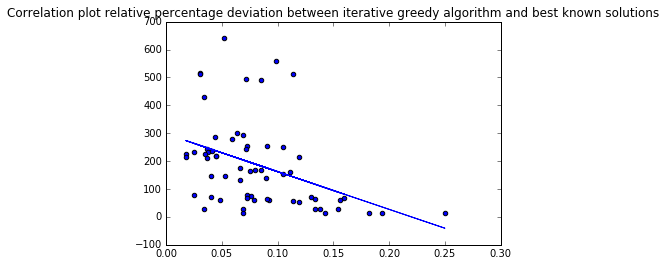
\includegraphics[width=\textwidth]{ig.png}
\end{figure}

\begin{figure}[p]
   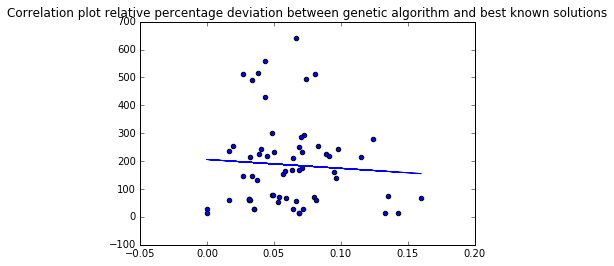
\includegraphics[width=\textwidth]{gen.png}
\end{figure}

A Wilcoxon test performed on the percentage deviation of the iterative greedy algorithm and the genetic algorithm to the best known values shows that we can reject the hypothesis that they are similar as the pvalue is 0.0015. 

When we compare the scores obtained with each of the algorithms to the best known scores, we obtain the same result, which lead us to conclude that the results are not accurate. The reason might be that the run-time duration was not long enough.


\subsubsection{Optimum}

Indeed the average percentage deviation is far less when the algorithm is let to run for longer in the hope of reaching the optimum. Unfortunately having only 4 values is too less to perform a test on the means as it would be biased by the lack of data.

On the four instances, the \textit{iterative greedy algorithm} obtains an average percentage deviation of 0.071, certainly because of its random nature that prevents it from finding global optima. 

Computation times for the iterative greedy algorithm : 
\begin{itemize}
    \item scpa1 : 10.002309083938599
    \item scpb1 : 10.003480672836304
    \item scpc1 : 14.007994890213013
    \item scpd1 : 15.004057168960571
\end{itemize}

Scores obtained by the iterative greedy algorithm : 

\begin{itemize}
    \item scpa1 : 272
    \item scpb1 : 81
    \item scpc1 : 235
    \item scpd1 : 63
\end{itemize}

The \textit{genetic algorithm} obtains an average percentage deviation of 0.048. On two of the instances, the algorithm is within the 2\% margin but on the two others it is less good.

Computation times for the genetic algorithm : 
\begin{itemize}
    \item scpa1 : 11.444749593734741
    \item scpb1 : 12.9664146900177
    \item scpc1 : 18.01086401939392
    \item scpd1 : 21.69332432746887
\end{itemize}

Scores obtained by the genetic algorithm : 

\begin{itemize}
    \item scpa1 : 258
    \item scpb1 : 78
    \item scpc1 : 234
    \item scpd1 : 61
\end{itemize}


\bibliography{main}
\end{document}
